% Don't Do That: Keep your data in line with database constraints
\documentclass{beamer}
\usetheme{Goettingen}

\begin{document}
\title{Don't Do That}
\subtitle{Ensuring data sanity with database constraints}
\author{Joshua Tolley\\
    End Point Corporation
}

\frame{\titlepage}
%\frame{\tableofcontents}

\begin{frame}
    Stuff I want to talk about
    \begin{itemize}
        \item ACID -- Describe consistency. Include examples
        \item Pitfalls of bad data -- more examples
        \item Different ways of managing constraints (indexes, constraints, triggers). Note that triggers don't validate already-entered data.
        \item Examples of index constraints (UNIQUE)
        \item column and table constraints (not null, check, default, unqiue, primary or foreign key. Example of multi-column foreign key
        \item cascading foreign keys
        \item Postgresql exclusion constraints
        \item triggers
        \item Refute Rails' "The app does it for me, so I don't have to worry about it in the database" agnosticism
    \end{itemize}
\end{frame}

%\begin{frame}
%"The degree of normality in a database is inversely proportional to that of its DBA."
%- Anon, twitter
%\end{frame}
%
%\section{Why and Why Not}
%\begin{frame}
%    \frametitle{Why Not Do Stuff in SQL}
%    \begin{itemize}
%        \item Databases are harder to replicate, if you \textbf{really} need to scale out
%        \pause
%        \begin{itemize}
%            \item Often, one complex SQL query is more efficient than several simple ones
%            \pause
%            \item Sometimes, indeed, it's useful to reduce the load on the database by moving logic into the application. Be careful doing this
%            \pause
%            \begin{itemize}
%                \item c.f. Premature Optimization
%                \pause
%            \end{itemize}
%        \end{itemize}
%        \item More complex queries are harder to write and debug
%        \pause
%        \begin{itemize}
%            \item True. But so is more complex programming.
%            \pause
%        \end{itemize}
%        \item More complex queries are harder for the next guy to maintain
%        \pause
%        \item Also, good DBAs are often more expensive than good programmers
%        \pause
%        \begin{itemize}
%            \item These are both true. But complex programming is also hard for the next guy to maintain
%            \pause
%            \item Of all the reasons not to write fluent SQL, this is probably the most widely applicable
%        \end{itemize}
%    \end{itemize}
%\end{frame}
%
%
%\begin{frame}
%    \frametitle{Why do stuff in SQL?}
%    \begin{itemize}
%        \item The database is more efficient than your application for processing big chunks of data
%        \pause
%        \begin{itemize}
%            \item ...especially if your code is in an interpreted language
%            \pause
%        \end{itemize}
%        \item The database is better tested than your application
%        \pause
%        \begin{itemize}
%            \item Applications trying to do what SQL should be doing often get big and complex quickly
%            \pause
%            \item ...and also buggy quickly 
%            \pause
%        \end{itemize}
%        \item That's what the database is there for
%        \pause
%        \item SQL is designed to express relations and conditions on them. Your application's language isn't.
%        \pause
%        \item A better understanding of SQL allows you to write queries that perform better
%    \end{itemize}
%\end{frame}
%
%\begin{frame}
%    \frametitle{Why do stuff in SQL?}
%    In short, the database exists to manage data, and your application exists to handle business logic. Write software accordingly.
%\end{frame}
%
%\begin{frame}
%    So let's get started...
%\end{frame}
%
%\begin{frame}[fragile]
%    \frametitle{Tables we'll use}
%
%   \begin{columns}[l]
%       \column{1.5in}
%       \begin{verbatim}
%# SELECT * FROM a;
% id | value
%----+-------
%  1 | a1
%  2 | a2
%  3 | a3
%  4 | a4
%(4 rows)
%       \end{verbatim}
%       \column{1.5in}
%       \begin{verbatim}
%# SELECT * FROM b;
% id | value
%----+-------
%  5 | b5
%  4 | b4
%  3 | b3
%  6 | b6
%(4 rows)
%       \end{verbatim}
%   \end{columns}
%\end{frame}
%
%\section{Joins}
%
%\begin{frame}
%    \frametitle{JOINs}
%    \begin{itemize}
%        \item If you want data from multiple tables, you probably want a join
%        \pause
%        \begin{itemize}
%            \item ...but see also Subqueries, later on
%            \pause
%        \end{itemize}
%        \item There are several different kinds of joins
%    \end{itemize}
%\end{frame}
%
%\begin{frame}[fragile]
%    \frametitle{JOINs}
%    \begin{verbatim}
%<table1> [alias1]
%    [ [ [NATURAL] [ [FULL | RIGHT | LEFT] [OUTER] |
%    INNER] ] | CROSS ] JOIN
%<table2> [alias2]
%    [USING (...) |
%    ON (<value1> <op> <value2>
%        [,<value3> <op> <value4>...] ) ]
%    \end{verbatim}
%\end{frame}
%
%\subsection{CROSS JOIN}
%
%\begin{frame}
%    \frametitle{CROSS JOIN}
%    \begin{itemize}
%        \item SELECT \textless ... \textgreater FROM table1 JOIN table2
%        \pause
%        \item With no explicit join type and no join qualifiers (an ON clause, WHERE clause involving both relations, etc.) this is a CROSS JOIN
%        \pause
%        \item Equivalent to
%        \begin{itemize}
%            \item SELECT \textless ... \textgreater FROM table1, table2
%            \pause
%            \item SELECT \textless ... \textgreater FROM table1 CROSS JOIN table2
%            \pause
%        \end{itemize}
%        \item "Cartesian product" of the two relations
%        \pause
%        \begin{itemize}
%            \item Combines every row of table1 with every row of table2
%            \pause
%            \item Makes \textbf{LOTS} of rows, and can thus be very slow
%        \end{itemize}
%    \end{itemize}
%\end{frame}
%
%\begin{frame}[fragile]
%    \frametitle{CROSS JOIN}
%    \begin{verbatim}
%# SELECT * FROM a, b;
% id | value | id | value
%----+-------+----+-------
%  1 | a1    |  5 | b5
%  1 | a1    |  4 | b4
%<snip>
%  3 | a3    |  3 | b3
%  3 | a3    |  6 | b6
%  4 | a4    |  5 | b5
%  4 | a4    |  4 | b4
%  4 | a4    |  3 | b3
%  4 | a4    |  6 | b6
%(16 rows)
%    \end{verbatim}
%\end{frame}
%
%\subsection{INNER JOIN}
%\begin{frame}
%    \frametitle{INNER JOIN}
%    \begin{itemize}
%        \item SELECT \textless ...\textgreater FROM table1 INNER JOIN table2 ON (table1.field = table2.field ...)
%        \pause
%        \item Only returns rows satisfying the ON condition
%        \pause
%        \item Equivalent to a CROSS JOIN with a WHERE clause
%    \end{itemize}
%\end{frame}
%
%\begin{frame}[fragile]
%    \frametitle{INNER JOIN}
%    \begin{verbatim}
%# SELECT * FROM a INNER JOIN b USING (id);
% id | value | value
%----+-------+-------
%  3 | a3    | b3
%  4 | a4    | b4
%(2 rows)
%    \end{verbatim}
%\end{frame}
%
%\subsection{OUTER JOIN}
%\begin{frame}
%    \frametitle{OUTER JOIN}
%    \begin{itemize}
%        \item Return all rows from one or both relations
%        \pause
%        \item LEFT: Return all rows from the relation on the left
%        \pause
%        \item RIGHT: Return all rows from the relation on the right
%        \pause
%        \item FULL: Return all rows from both relations
%        \pause
%        \item Returns nulls for values from one relation when it contains to match with the other relation
%        \pause
%        \item The OUTER keyword is redundant
%        \pause
%        \item Requires ON or USING clause
%    \end{itemize}
%\end{frame}
%
%\begin{frame}[fragile]
%    \frametitle{LEFT JOIN}
%    \begin{verbatim}
%# SELECT * FROM a LEFT JOIN b USING (id);
% id | value | value
%----+-------+-------
%  1 | a1    |
%  2 | a2    |
%  3 | a3    | b3
%  4 | a4    | b4
%(4 rows)
%    \end{verbatim}
%\end{frame}
%
%\begin{frame}[fragile]
%    \frametitle{RIGHT JOIN}
%    \begin{verbatim}
%# SELECT * FROM a RIGHT JOIN b USING (id);
% id | value | value
%----+-------+-------
%  3 | a3    | b3
%  4 | a4    | b4
%  5 |       | b5
%  6 |       | b6
%(4 rows)
%    \end{verbatim}
%\end{frame}
%
%\begin{frame}[fragile]
%    \frametitle{FULL JOIN}
%    \begin{verbatim}
%# select * from a full join b using (id);
% id | value | value
%----+-------+-------
%  1 | a1    |
%  2 | a2    |
%  3 | a3    | b3
%  4 | a4    | b4
%  5 |       | b5
%  6 |       | b6
%(6 rows)
%    \end{verbatim}
%\end{frame}
%
%\begin{frame}[fragile]
%    \frametitle{Applications}
%    Find rows with no match in table b: \\
%    \begin{verbatim}
%# SELECT * FROM a LEFT JOIN b USING (id)
%    WHERE b.value IS NULL;
% id | value | value
%----+-------+-------
%  1 | a1    |
%  2 | a2    |
%(2 rows)
%    \end{verbatim}
%\end{frame}
%
%\subsection{NATURAL JOIN}
%\begin{frame}
%    \frametitle{NATURAL JOIN}
%    \begin{itemize}
%        \item NATURAL is syntactic sugar to match all columns with the same name
%    \end{itemize}
%\end{frame}
%
%\begin{frame}[fragile]
%    \frametitle{NATURAL JOIN}
%    \begin{verbatim}
%# SELECT * FROM a NATURAL FULL JOIN b;
% id | value
%----+-------
%  1 | a1
%  2 | a2
%  3 | a3
%  3 | b3
%  4 | a4
%  4 | b4
%  5 | b5
%  6 | b6
%(8 rows)
%    \end{verbatim}
%%    \vspace{10pt}
%    This looked for matches in both the \emph{id} and \emph{value} columns, so no rows matched. It returned all rows of both relations because it's a FULL JOIN.
%\end{frame}
%
%\subsection{Self Joins}
%\begin{frame}
%    \frametitle{Self Joins}
%    \begin{itemize}
%        \item "Self joins" are particularly counterintuitive
%        \pause
%        \item Joins one table to itself
%        \pause
%        \item It helps to give the table two different aliases
%    \end{itemize}
%\end{frame}
%
%\begin{frame}[fragile]
%    \frametitle{Self Joins}
%    Find all employees' names, and each employee's manager
%    %\vspace{10pt}
%    \begin{verbatim}
%SELECT
%    e.first || ' ' || e.last,
%    (SELECT
%        m.first || ' ' || m.last
%     FROM employee m
%     WHERE m.id = e.manager);
%    \end{verbatim}
%    %\vspace{10pt}
%    ... will generally be much faster rewritten as ...
%    %\vspace{10pt}
%    \begin{verbatim}
%SELECT
%    e.first || ' ' || e.last,
%    m.first || ' ' || m.last
%FROM
%    employee e
%    JOIN employee m ON (e.manager = m.id)
%    \end{verbatim}
%    %\vspace{10pt}
%\end{frame}
%
%\section{Other Useful Operations}
%\begin{frame}
%    More useful operations...
%\end{frame}
%
%\subsection{Subqueries}
%\begin{frame}
%    \frametitle{Subqueries}
%    \begin{itemize}
%        \item Embeds one query within another
%        \pause
%        \item Examples (some bad, some good)
%        \pause
%        \begin{itemize}
%            \item SELECT id FROM table WHERE field = (SELECT MAX(field) FROM table)
%            \pause
%            \item SELECT id, (SELECT COUNT(*) FROM table2 WHERE id = table1.id) FROM table1
%            \pause
%            \item SELECT a, b FROM (SELECT a, COUNT(*) AS c FROM table1) t1 JOIN (SELECT b, COUNT(*) AS c FROM table2) t2 on (t1.c = t2.c)
%            \pause
%            \begin{itemize}
%                \item You can join subqueries just like you'd join tables
%            \end{itemize}
%        \end{itemize}
%    \end{itemize}
%\end{frame}
%
%\subsection{Set Operations}
%\begin{frame}
%    \frametitle{Set Operations}
%    \begin{itemize}
%        \item INTERSECT
%        \pause
%        \begin{itemize}
%            \item Returns the intersection of two sets
%            \pause
%            \item Doesn't exist in MySQL
%            \pause
%            \item SELECT (SELECT a, b FROM table1) INTERSECT (SELECT c, d FROM table2)
%            \pause
%        \end{itemize}
%        \item UNION
%        \pause
%        \begin{itemize}
%            \item Appends one set of rows to another set with matching column types
%            \pause
%            \item SELECT a FROM table1 UNION SELECT b FROM table2
%            \pause
%        \end{itemize}
%        \item EXCEPT
%        \pause
%        \begin{itemize}
%            \item Returns rows in one SELECT that aren't in another SELECT
%            \pause
%            \item SELECT a FROM table1 EXCEPT SELECT b FROM table2
%        \end{itemize}
%    \end{itemize}
%\end{frame}
%
%\subsection{Common Operations}
%\begin{frame}
%    \frametitle{Common Operations}
%    \begin{itemize}
%        \item COALESCE(a, b)
%        \pause
%        \begin{itemize}
%            \item If \texttt{a} is null, return \texttt{b}, else return \texttt{a}
%            \pause
%            \item SELECT COALESCE(first, '\textless NULL\textgreater ') FROM table
%            \pause
%            \item Oracle calls this NVL()
%            \pause
%        \end{itemize}
%        \item CASE...WHEN
%        \pause
%        \begin{itemize}
%            \item Conditional operation
%            \pause
%            \item SELECT CASE WHEN langused IN ('Lisp', 'OCaml', 'Haskell') THEN 'Functional' ELSE 'Imperative' AS langtype FROM software
%        \end{itemize}
%    \end{itemize}
%\end{frame}
%
%\begin{frame}[fragile]
%    \frametitle{Series Generation}
%    \begin{itemize}
%        \item generate\_series() in PostgreSQL; might be something else in other databases
%        \pause
%        \item Returns a series of numbers
%        \pause
%        \item Can be used like a \texttt{for} loop (example given later)
%    \end{itemize}
%    \begin{verbatim}
%# SELECT * FROM generate_series(1, 5);
% generate_series
%-----------------
%               1
%               2
%               3
%               4
%               5
%(5 rows)
%    \end{verbatim}
%\end{frame}
%
%\section{Advanced Operations}
%\subsection{Common Table Expressions}
%\begin{frame}
%    \frametitle{Common Table Expressions}
%    \begin{itemize}
%        \item Abbreviated CTEs
%        \pause
%        \item Fairly advanced; not available in all databases
%        \pause
%        \begin{itemize}
%            \item Not in PostgreSQL before v. 8.4, or any version of MySQL
%        \end{itemize}
%        \item It's just like defining a one-time view for your query
%        \pause
%        \item One major benefit: CTEs allow recursion
%        \pause
%        \begin{itemize}
%            \item Recursing with CTEs is much more efficent than processing recursive data in your application
%        \end{itemize}
%    \end{itemize}
%\end{frame}
%
%\begin{frame}[fragile]
%    \frametitle{A Simple CTE Example}
%    \begin{verbatim}
%# SELECT * FROM GENERATE_SERIES(1,3)
%CROSS JOIN
%    (SELECT * FROM GENERATE_SERIES(8,9)) AS f;
% generate_series | generate_series
%-----------------+-----------------
%               1 |               8
%               1 |               9
%               2 |               8
%               2 |               9
%               3 |               8
%               3 |               9
%(6 rows)
%    \end{verbatim}
%\end{frame}
%
%\begin{frame}[fragile]
%    \frametitle{A Simple CTE Example}
%    \begin{verbatim}
%# WITH t AS (
%    SELECT * FROM GENERATE_SERIES(8,9)
%)
%SELECT * FROM GENERATE_SERIES(1,3)
%CROSS JOIN t;
% generate_series | generate_series
%-----------------+-----------------
%               1 |               8
%               1 |               9
%               2 |               8
%               2 |               9
%               3 |               8
%               3 |               9
%(6 rows)
%    \end{verbatim}
%\end{frame}
%
%\begin{frame}
%    \begin{center}
%    That last example was a bit cheesy, but the technique can be useful for complex queries in several parts
%    \end{center}
%\end{frame}
%
%\begin{frame}[fragile]
%    \frametitle{Recursion}
%    Start with this:
%    \begin{verbatim}
%# SELECT * FROM employee;
% first  |   last   | id | manager
%--------+----------+----+---------
% john   | doe      |  1 |
% fred   | rogers   |  2 |       1
% speedy | gonzales |  3 |       1
% carly  | fiorina  |  4 |       1
% hans   | reiser   |  5 |       2
% johnny | carson   |  6 |       5
% martha | stewart  |  7 |       3
%(7 rows)
%    \end{verbatim}
%\end{frame}
%
%\begin{frame}[fragile]
%    \frametitle{Recursion}
%    Recursive CTE to retrieve management hierarchy:
%    \begin{verbatim}
%# WITH RECURSIVE t (id, managernames) AS (
%    SELECT e.id, first || ' ' || last
%        AS managernames
%    FROM employee e WHERE manager IS NULL
%        UNION ALL
%    SELECT e.id,
%    first || ' ' || last || ', ' || managernames
%        AS managernames
%    FROM employee e
%    JOIN t ON (e.manager = t.id)
%    WHERE manager IS NOT NULL
%)
%SELECT e.id, first || ' ' || last AS name,
%    managernames
%FROM employee e JOIN t ON (e.id = t.id);
%    \end{verbatim}
%\end{frame}
%
%\begin{frame}[fragile]
%    \frametitle{Recursion}
%    ...and get this...
%    \begin{verbatim}
% id |     name        |  managernames                   
%----+-----------------+-----------------------------
%  1 | john doe        | john doe
%  2 | fred rogers     | fred rogers, john doe
%  3 | speedy gonzales | speedy gonzales, john doe
%  4 | carly fiorina   | carly fiorina, john doe
%  5 | hans reiser     | hans reiser, fred rogers,
%    |                 |  john doe
%  6 | johnny carson   | johnny carson, hans reiser,
%    |                 |  fred rogers, john doe
%  7 | martha stewart  | martha stewart, speedy
%    |                 |  gonzales, john doe
%(7 rows)
%    \end{verbatim}
%\end{frame}
%
%\begin{frame}[fragile]
%    \frametitle{Fractals in SQL}
%    \tiny
%    \begin{verbatim}
%WITH RECURSIVE x(i) AS
%(VALUES(0) UNION ALL SELECT i + 1 FROM x WHERE i < 101),
%Z(Ix, Iy, Cx, Cy, X, Y, I)
%AS (
%    SELECT Ix, Iy, X::float, Y::float, X::float, Y::float, 0
%    FROM (SELECT -2.2 + 0.031 * i, i FROM x) AS xgen(x,ix)
%        CROSS JOIN
%    (SELECT -1.5 + 0.031 * i, i FROM x) AS ygen(y,iy)
%        UNION ALL
%    SELECT
%        Ix, Iy, Cx, Cy, X * X - Y * Y + Cx AS X,
%        Y * X * 2 + Cy, I + 1
%    FROM Z
%    WHERE X * X + Y * Y < 16.0 AND I < 27),
%Zt (Ix, Iy, I) AS (
%    SELECT Ix, Iy, MAX(I) AS I
%    FROM Z GROUP BY Iy, Ix
%    ORDER BY Iy, Ix
%)
%SELECT array_to_string(
%    array_agg(
%        SUBSTRING(' .,,,-----++++%%%%@@@@#### ',
%            GREATEST(I,1), 1)
%    ),''
%)
%FROM Zt GROUP BY Iy ORDER BY Iy;
%    \end{verbatim}
%    \normalsize
%    (yes, this query is SQL-spec compliant)
%\end{frame}
%
%\begin{frame}
%    \scalebox{.3}{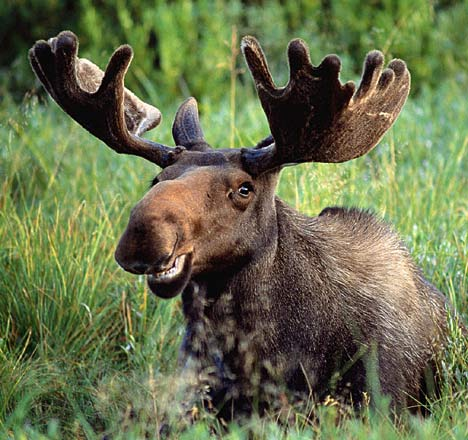
\includegraphics{mandelbrot.png}}
%\end{frame}
%
%\subsection{Window Functions}
%\begin{frame}
%    \frametitle{Window Functions}
%    \begin{itemize}
%        \item Like CTEs, these are quite advanced
%        \pause
%        \item Also unavailable in MySQL, and PostgreSQL before 8.4
%        \pause
%        \item Allow ranking, moving averages
%        \pause
%        \item Like a set-returning aggregate function. Window functions return results for each row based on a "window" of related rows
%    \end{itemize}
%\end{frame}
%
%\begin{frame}[fragile]
%    \frametitle{Window Functions}
%    If our employee table had department and salary information...
%    \begin{verbatim}
%# SELECT first, last, salary, department
%    FROM employee;
% first  |   last   | salary |   department
%--------+----------+--------+----------------
% fred   | rogers   |  97000 | sales
% carly  | fiorina  |  95000 | sales
% johnny | carson   |  89000 | sales
% speedy | gonzales |  96000 | development
% hans   | reiser   |  93000 | development
% martha | stewart  |  90000 | development
% john   | doe      |  99000 | administration
%(7 rows)
%    \end{verbatim}
%\end{frame}
%
%\begin{frame}[fragile]
%    \frametitle{Window Functions Example}
%    Rank employees in each department by salary
%    \begin{verbatim}
%SELECT first, last, salary, department,
%    RANK() OVER (
%        PARTITION BY department
%        ORDER BY salary DESC
%    )
%FROM employee
%    \end{verbatim}
%\end{frame}
%
%\begin{frame}[fragile]
%    \frametitle{Window Functions Example}
%    ... and get this:
%    \footnotesize
%    \begin{verbatim}
% first  |   last   | salary |   department   | rank
%--------+----------+--------+----------------+------
% john   | doe      |  99000 | administration |    1
% speedy | gonzales |  96000 | development    |    1
% hans   | reiser   |  93000 | development    |    2
% martha | stewart  |  90000 | development    |    3
% fred   | rogers   |  97000 | sales          |    1
% carly  | fiorina  |  95000 | sales          |    2
% johnny | carson   |  89000 | sales          |    3
%(7 rows)
%    \end{verbatim}
%    \normalsize
%\end{frame}
%
%\section{Real, Live Queries}
%\subsection{Something Simple}
%\begin{frame}
%    \begin{center}
%       Real, live queries
%    \end{center}
%\end{frame}
%
%\begin{frame}[fragile]
%    \frametitle{Something Simple}
%    The slow version:
%    \begin{verbatim}
%SELECT DISTINCT(sync) FROM bucardo.bucardo_rate
%ORDER BY 1
%    \end{verbatim}
%    The fast version:
%    \begin{verbatim}
%SELECT name FROM sync WHERE EXISTS (
%    SELECT 1 FROM bucardo_rate
%    WHERE sync = name LIMIT 1)
%ORDER BY 1
%    \end{verbatim}
%\end{frame}
%
%\begin{frame}
%    \frametitle{Something Simple}
%    \begin{itemize}
%        \item The \emph{bucardo\_rate} table is huge, with few distinct values
%        \pause
%        \item finding "DISTINCT sync" requires a \textbf{\emph{long}} table scan
%        \pause
%        \item The \emph{sync} table contains a list of all possible values in the \emph{bucardo\_rate.sync} column
%        \pause
%        \item So instead of a big table scan, we scan the small table, and filter out values can't find in \emph{bucardo\_rate}
%    \end{itemize}
%\end{frame}
%
%\subsection{Something Fun}
%\begin{frame}
%    \begin{center}Something Fun\end{center}
%\end{frame}
%
%\begin{frame}[fragile]
%    \tiny
%    \begin{verbatim}
%SELECT
%    id, idname,
%    COALESCE(ROUND(AVG(synctime)::NUMERIC, 1), 0) AS avgtime,
%    COALESCE(SUM(total), 0) AS count
%FROM (
%    SELECT slavecommit,
%    EXTRACT(EPOCH FROM slavecommit - mastercommit) AS synctime,
%    total
%    FROM bucardo.bucardo_rate
%    WHERE sync = 'RO_everything' AND
%    mastercommit > (NOW() - (15 + 1) * INTERVAL '1 HOUR')
%) i
%RIGHT JOIN (
%    SELECT id, idname,
%        TO_TIMESTAMP(start - start::INTEGER % 3600) AS start,
%        TO_TIMESTAMP(stop - stop::INTEGER % 3600) AS stop
%    FROM (
%        SELECT id,
%            TO_CHAR(NOW() - id * INTERVAL '1 HOUR', 
%                'Dy Mon DD HH:MI AM') AS idname,
%            EXTRACT(EPOCH FROM NOW() - id * INTERVAL '1 HOUR') AS start,
%            EXTRACT(EPOCH FROM NOW() - (id - 1) * INTERVAL '1 HOUR') AS stop
%        FROM (
%            SELECT GENERATE_SERIES(1, 15) AS id
%        ) f
%    ) g
%) h ON (slavecommit BETWEEN start AND stop)
%GROUP BY id, idname
%ORDER BY id DESC;
%    \end{verbatim}
%\end{frame}
%
%\begin{frame}
%    \frametitle{Something Fun}
%    \begin{itemize}
%        \item The table contains replication data
%        \pause
%        \begin{itemize}
%            \item Time of commit on master
%            \pause
%            \item Time of commit on slave
%            \pause
%            \item Number of rows replicated
%            \pause
%        \end{itemize}
%        \item The user wants a graph of replication speed over time, given a user-determined range of time
%    \end{itemize}
%\end{frame}
%
%\begin{frame}[fragile]
%    \frametitle{Something Fun}
%    We want to average replication times over a series of buckets. The first
%    part of our query creates those buckets, based on
%    \texttt{generate\_series()}. Here we create buckets for 15 hours
%    \begin{verbatim}
%SELECT 
%    id,
%    TO_CHAR(NOW() - id * INTERVAL '1 HOUR',
%        'Dy Mon DD HH:MI AM') AS idname,
%    EXTRACT(EPOCH FROM NOW() - id *
%        INTERVAL '1 HOUR') AS start,
%    EXTRACT(EPOCH FROM NOW() - (id - 1) *
%        INTERVAL '1 HOUR') AS stop
%FROM (
%    SELECT GENERATE_SERIES(1, 15) AS id
%) f
%    \end{verbatim}
%\end{frame}
%
%\begin{frame}[fragile]
%    \frametitle{Something Fun}
%    This gives us:
%    \scriptsize
%    \begin{verbatim}
% id |       idname        |      start       |       stop
%----+---------------------+------------------+------------------
%  1 | Sat Mar 14 10:23 PM | 1237091036.95657 | 1237094636.95657
%  2 | Sat Mar 14 09:23 PM | 1237087436.95657 | 1237091036.95657
%  3 | Sat Mar 14 08:23 PM | 1237083836.95657 | 1237087436.95657
%  4 | Sat Mar 14 07:23 PM | 1237080236.95657 | 1237083836.95657
%...
%    \end{verbatim}
%    \normalsize
%\end{frame}
%
%\begin{frame}[fragile]
%    \frametitle{Something Fun}
%    Make the buckets end on nice time boundaries:
%    \begin{verbatim}
%SELECT id, idname,
%    TO_TIMESTAMP(start - start::INTEGER % 3600)
%        AS start,
%    TO_TIMESTAMP(stop - stop::INTEGER % 3600)
%        AS stop
%FROM (
%    -- The bucket query, shown earlier, goes here
%) g
%    \end{verbatim}
%\end{frame}
%
%\begin{frame}[fragile]
%    \frametitle{Something Fun}
%    That gives us this:
%    \tiny
%    \begin{verbatim}
% id |       idname        |             start             |             stop
%----+---------------------+-------------------------------+-------------------------------
%  1 | Sat Mar 14 10:23 PM | 2009-03-14 21:59:59.956568-06 | 2009-03-14 22:59:59.956568-06
%  2 | Sat Mar 14 09:23 PM | 2009-03-14 20:59:59.956568-06 | 2009-03-14 21:59:59.956568-06
%  3 | Sat Mar 14 08:23 PM | 2009-03-14 19:59:59.956568-06 | 2009-03-14 20:59:59.956568-06
%  4 | Sat Mar 14 07:23 PM | 2009-03-14 18:59:59.956568-06 | 2009-03-14 19:59:59.956568-06
%    \end{verbatim}
%    \normalsize
%\end{frame}
%
%\begin{frame}[fragile]
%    \frametitle{Something Fun}
%    In an different subquery, select everything from the table of the right
%    time period and right sync. Call this the "stats" query:
%    \begin{verbatim}
%SELECT
%    slavecommit,
%    EXTRACT(EPOCH FROM slavecommit - mastercommit)
%        AS synctime,
%    total
%FROM bucardo.bucardo_rate
%WHERE
%    sync = 'RO_everything' AND
%    mastercommit > (NOW() - (15 + 1) *
%        INTERVAL '1 HOUR')
%    \end{verbatim}
%\end{frame}
%
%\begin{frame}[fragile]
%    \frametitle{Something Fun}
%    ...which gives us this:
%    \footnotesize
%    \begin{verbatim}
%          slavecommit          |     synctime     | total
%-------------------------------+------------------+--------
% 2009-03-14 07:32:00.103759-06 | 5.65614098310471 |      1
% 2009-03-14 07:32:04.31508-06  | 5.25827997922897 |      3
% 2009-03-14 07:32:04.31508-06  | 5.25827997922897 |      5
% 2009-03-14 07:32:08.700184-06 | 7.71899098157883 |      1
% 2009-03-14 07:32:08.700184-06 | 8.22490698099136 |      1
% 2009-03-14 07:32:12.675518-06 | 7.85176599025726 |      6
% 2009-03-14 07:32:12.675518-06 | 7.15798497200012 |      6
%...
%    \end{verbatim}
%    \normalsize
%\end{frame}
%
%\begin{frame}[fragile]
%    \frametitle{Something Fun}
%    Now, join the two queries:
%    \begin{verbatim}
%SELECT
%    id, idname,
%    COALESCE(ROUND(AVG(synctime)::NUMERIC, 1), 0)
%        AS avgtime,
%    COALESCE(SUM(total), 0) AS count
%FROM (
%    <STATS QUERY>
%)  RIGHT JOIN (
%    <CALENDAR QUERY>
%) ON (slavecommit BETWEEN start AND stop)
%GROUP BY id, idname
%ORDER BY id DESC;
%    \end{verbatim}
%\end{frame}
%
%\begin{frame}[fragile]
%    \frametitle{Something Fun}
%    ...and get this:
%    \begin{verbatim}
% id |       idname        | avgtime | count
%----+---------------------+---------+-------
% 15 | Sat Mar 14 08:35 AM |     7.9 | 14219
% 14 | Sat Mar 14 09:35 AM |     6.9 | 16444
% 13 | Sat Mar 14 10:35 AM |     6.5 | 62100
% 12 | Sat Mar 14 11:35 AM |     6.2 | 47349
% 11 | Sat Mar 14 12:35 PM |       0 |     0
% 10 | Sat Mar 14 01:35 PM |     4.6 | 21348
%    \end{verbatim}
%    This is the average replication time and total replicated rows per hour.
%    Note that this correctly returns zeroes when no rows are replicated, and
%    still returns a value for that time slot. This prevents some amount of
%    application-side processing.
%\end{frame}
%
%\begin{frame}
%    \frametitle{Something Fun}
%    \center{That query again:}
%\end{frame}
%
%\begin{frame}[fragile]
%    \tiny
%    \begin{verbatim}
%SELECT
%    id, idname,
%    COALESCE(ROUND(AVG(synctime)::NUMERIC, 1), 0) AS avgtime,
%    COALESCE(SUM(total), 0) AS count
%FROM (
%    SELECT slavecommit,
%    EXTRACT(EPOCH FROM slavecommit - mastercommit) AS synctime,
%    total
%    FROM bucardo.bucardo_rate
%    WHERE sync = 'RO_everything' AND
%    mastercommit > (NOW() - (15 + 1) * INTERVAL '1 HOUR')
%) i
%RIGHT JOIN (
%    SELECT id, idname,
%        TO_TIMESTAMP(start - start::INTEGER % 3600) AS start,
%        TO_TIMESTAMP(stop - stop::INTEGER % 3600) AS stop
%    FROM (
%        SELECT id,
%            TO_CHAR(NOW() - id * INTERVAL '1 HOUR', 
%                'Dy Mon DD HH:MI AM') AS idname,
%            EXTRACT(EPOCH FROM NOW() - id * INTERVAL '1 HOUR') AS start,
%            EXTRACT(EPOCH FROM NOW() - (id - 1) * INTERVAL '1 HOUR') AS stop
%        FROM (
%            SELECT GENERATE_SERIES(1, 15) AS id
%        ) f
%    ) g
%) h ON (slavecommit BETWEEN start AND stop)
%GROUP BY id, idname
%ORDER BY id DESC;
%    \end{verbatim}
%\end{frame}
%
%\section{Key Points}
%\begin{frame}
%    \frametitle{Key Points}
%    \begin{itemize}
%        \item Understand join types, and use them
%        \pause
%        \item Know what functions and set operations your database provides
%        \pause
%        \item Build large queries piece by piece
%    \end{itemize}
%\end{frame}
%
%\frame{Questions?}
%
\end{document}
